\documentclass[10pt]{extarticle}

\usepackage[brazilian]{babel}
\usepackage{graphicx}
\usepackage{float}
\usepackage{booktabs}
\usepackage{multirow}
\usepackage{framed}
\usepackage[normalem]{ulem}
\usepackage{indentfirst}
\usepackage{varwidth}
\usepackage{amsmath,amsthm,amssymb,amsfonts}
\usepackage{mathtools} % Wraparound amsmath. For fancy math typesetting
\usepackage[nointegrals]{wasysym} % nointegrals prevents wasysym from overwriting integral symbols from LaTeX and amsmath
\usepackage{bbm} % For extended bold and blackboard bold characters
\usepackage[italicdiff]{physics} % italicdiff causes derivatives to be rendered with italic d's instead of upright d's
\usepackage[T1]{fontenc}
\usepackage{xparse}
\usepackage{tasks}
\usepackage{xstring}
% \usepackage{pifont} % For unusual symbols
% \usepackage{mathdots} % For unusual combinations of dots
\usepackage{wrapfig}
\usepackage{lmodern,mathrsfs}
\usepackage[inline,shortlabels]{enumitem}
\setlist{topsep=2pt,itemsep=2pt,parsep=0pt,partopsep=0pt}
\usepackage[table,dvipsnames]{xcolor}
\usepackage[utf8]{inputenc}
\usepackage{csquotes} % Must be loaded AFTER inputenc
\usepackage[a4paper,top=0.5in,bottom=0.2in,left=0.5in,right=0.5in,footskip=0.3in,includefoot]{geometry}
\usepackage{setspace}
\usepackage[most]{tcolorbox}
\usepackage{tikz,tkz-base, tkz-fct,tikz-3dplot,tikz-cd,tkz-tab,tkz-euclide,pgf,pgfplots}
\usepackage{pstricks}
\usepackage{pst-plot}
\pgfplotsset{compat=newest}
% \usepackage{comment} % For commenting large blocks of text and math efficiently
% \usepackage{fancyvrb} % For custom verbatim environments
\usepackage{multicol}
\usetikzlibrary{matrix,arrows,decorations.pathmorphing}
\usepackage{systeme}
\usepackage{verbatim}
\usepackage[bottom,multiple]{footmisc} % Ensures footnotes are at the bottom of the page, and separates footnotes by a comma if they are adjacent
% \usepackage[backend=bibtex,style=numeric]{biblatex}
% \renewcommand*{\finalnamedelim}{\addcomma\addspace} % Forces authors' names to be separated by comma, instead of "and"
% \addbibresource{bibliography}
\usepackage[colorlinks,linkcolor=.,citecolor=blue,urlcolor=violet]{hyperref}
\usepackage[nameinlink]{cleveref} % nameinlink ensures that the entire element is clickable in the pdf, not just the number

\newcommand{\tm}{^{\mathsf{T}}}     % Transpose
\newcommand{\hm}{^{\mathsf{H}}}     % Conjugate transpose (Hermitian conjugate)
\newcommand{\itm}{^{-\mathsf{T}}}   % Inverse transpose
\newcommand{\ihm}{^{-\mathsf{H}}}   % Inverse conjugate transpose (Inverse Hermitian conjugate)

\newtheoremstyle{mystyle}{}{}{}{}{\sffamily\bfseries}{.}{ }{}
\makeatletter
\renewenvironment{proof}[1][\proofname] {\par\pushQED{\qed}{\normalfont\sffamily\bfseries\topsep6\p@\@plus6\p@\relax #1\@addpunct{.} }}{\popQED\endtrivlist\@endpefalse}
\makeatother
\renewcommand{\qedsymbol}{\coolqed{0.32}} % Implements the new QED symbol
\theoremstyle{mystyle}{\newtheorem*{remark}{Remark}}
\theoremstyle{mystyle}{\newtheorem*{remarks}{Remarks}}
\theoremstyle{mystyle}{\newtheorem*{example}{Exemplo}}
\theoremstyle{mystyle}{\newtheorem*{examples}{Exemplos}}
\theoremstyle{definition}{\newtheorem*{exercise}{Exercício Resolvido}}

% Warning environment
\newtheoremstyle{warn}{}{}{}{}{\normalfont}{}{ }{}
\theoremstyle{warn}
\newtheorem*{warning}{\warningsign{0.2}\relax}

% Symbol for the warning environment, designed to be easily scalable
\newcommand{\warningsign}[1]{
    \tikz[scale=#1,every node/.style={transform shape}]{
        \draw[-,line width={#1*0.8mm},red,fill=yellow,rounded corners={#1*2.5mm}] (0,0)--(1,{-sqrt(3)})--(-1,{-sqrt(3)})--cycle;
        \node at (0,-1) {\fontsize{48}{60}\selectfont\bfseries!};
}}

\newcommand{\coolqed}[1]{\includegraphics[width=#1cm]{sunglasses_emoji.png}} % QED symbol

\newtcbtheorem[number within=section]{Definition}{Definition}{enhanced,
	before skip=2mm,after skip=2mm, colback=red!5,colframe=red!80!black,boxrule=0.5mm,
	attach boxed title to top left={xshift=1cm,yshift*=1mm-\tcboxedtitleheight}, varwidth boxed title*=-3cm,
	boxed title style={frame code={
					\path[fill=tcbcolback]
					([yshift=-1mm,xshift=-1mm]frame.north west)
					arc[start angle=0,end angle=180,radius=1mm]
					([yshift=-1mm,xshift=1mm]frame.north east)
					arc[start angle=180,end angle=0,radius=1mm];
					\path[left color=tcbcolback!60!black,right color=tcbcolback!60!black,
						middle color=tcbcolback!80!black]
					([xshift=-2mm]frame.north west) -- ([xshift=2mm]frame.north east)
					[rounded corners=1mm]-- ([xshift=1mm,yshift=-1mm]frame.north east)
					-- (frame.south east) -- (frame.south west)
					-- ([xshift=-1mm,yshift=-1mm]frame.north west)
					[sharp corners]-- cycle;
				},interior engine=empty,
		},
	fonttitle=\bfseries,
	title={#2},#1}{def}

%================================
% NOTE BOX
%================================

\usetikzlibrary{arrows,calc,shadows.blur}
\tcbuselibrary{skins}
\newtcolorbox{note}[1][]{%
	enhanced jigsaw,
	colback=gray!20!white,%
	colframe=gray!80!black,
	size=small,
	boxrule=1pt,
	title=\textbf{Nota:-},
	halign title=flush center,
	coltitle=black,
	breakable,
	drop shadow=black!50!white,
	attach boxed title to top left={xshift=1cm,yshift=-\tcboxedtitleheight/2,yshifttext=-\tcboxedtitleheight/2},
	minipage boxed title=1.5cm,
	boxed title style={%
			colback=white,
			size=fbox,
			boxrule=1pt,
			boxsep=2pt,
			underlay={%
					\coordinate (dotA) at ($(interior.west) + (-0.5pt,0)$);
					\coordinate (dotB) at ($(interior.east) + (0.5pt,0)$);
					\begin{scope}
						\clip (interior.north west) rectangle ([xshift=3ex]interior.east);
						\filldraw [white, blur shadow={shadow opacity=60, shadow yshift=-.75ex}, rounded corners=2pt] (interior.north west) rectangle (interior.south east);
					\end{scope}
					\begin{scope}[gray!80!black]
						\fill (dotA) circle (2pt);
						\fill (dotB) circle (2pt);
					\end{scope}
				},
		},
	#1,
}
\newcommand{\nt}[1]{\begin{note}#1\end{note}}
\newcommand{\dfn}[3][]{\begin{Definition}[colbacktitle=red!75!black]{#2}{#1}#3\end{Definition}}


\definecolor{tcol_DEF}{HTML}{E40125} % Color for Definition
\definecolor{tcol_PRP}{HTML}{EB8407} % Color for Proposition
\definecolor{tcol_LEM}{HTML}{05C4D9} % Color for Lemma
\definecolor{tcol_THM}{HTML}{1346E4} % Color for Theorem
\definecolor{tcol_COR}{HTML}{7904C2} % Color for Corollary
\definecolor{tcol_REM}{HTML}{18B640} % Color for Remark
\definecolor{tcol_PRF}{HTML}{5A76B2} % Color for Proof
\definecolor{tcol_EXA}{HTML}{21340A} % Color for Example

\tcbset{
tbox_DEF_style/.style={enhanced jigsaw,
    colback=tcol_DEF!10,colframe=tcol_DEF!80!black,,
    fonttitle=\sffamily\bfseries,
    separator sign=.,label separator={},
    sharp corners,top=2pt,bottom=2pt,left=2pt,right=2pt,
    before skip=10pt,after skip=10pt,breakable
},
tbox_PRP_style/.style={enhanced jigsaw,
    colback=tcol_PRP!10,colframe=tcol_PRP!80!black,
    fonttitle=\sffamily\bfseries,
    attach boxed title to top left={yshift=-\tcboxedtitleheight},
    boxed title style={
        boxrule=0pt,boxsep=2.5pt,
        colback=tcol_PRP!80!black,colframe=tcol_PRP!80!black,
        sharp corners=uphill
    },
    separator sign=.,label separator={},
    top=\tcboxedtitleheight,bottom=2pt,left=2pt,right=2pt,
    before skip=10pt,after skip=10pt,drop fuzzy shadow,breakable
},
tbox_THM_style/.style={enhanced jigsaw,
    colback=tcol_THM!10,colframe=tcol_THM!80!black,
    fonttitle=\sffamily\bfseries,coltitle=black,
    attach boxed title to top left={xshift=10pt,yshift=-\tcboxedtitleheight/2},
    boxed title style={
        colback=tcol_THM!10,colframe=tcol_THM!80!black,height=16pt,bean arc
    },
    separator sign=.,label separator={},
    sharp corners,top=6pt,bottom=2pt,left=2pt,right=2pt,
    before skip=10pt,after skip=10pt,breakable
},
tbox_LEM_style/.style={enhanced jigsaw,
    colback=tcol_LEM!10,colframe=tcol_LEM!80!black,
    boxrule=0pt,
    fonttitle=\sffamily\bfseries,
    attach boxed title to top left={yshift=-\tcboxedtitleheight},
    boxed title style={
        boxrule=0pt,boxsep=2pt,
        colback=tcol_LEM!80!black,colframe=tcol_LEM!80!black,
        interior code={\fill[tcol_LEM!80!black] (interior.north west)--(interior.south west)--([xshift=-2mm]interior.south east)--([xshift=2mm]interior.north east)--cycle;
    }},
    separator sign=.,label separator={},
    frame hidden,borderline north={1pt}{0pt}{tcol_LEM!80!black},
    before upper={\hspace{\tcboxedtitlewidth}},
    sharp corners,top=2pt,bottom=2pt,left=5pt,right=5pt,
    before skip=10pt,after skip=10pt,breakable
},
tbox_COR_style/.style={enhanced jigsaw,
    colback=tcol_COR!10,colframe=tcol_COR!80!black,
    boxrule=0pt,
    fonttitle=\sffamily\bfseries,coltitle=black,
    separator sign={},label separator={},
    description font=\normalfont\sffamily,
    description delimiters={(}{)},
    attach title to upper,after title={.\ },
    frame hidden,borderline west={2pt}{0pt}{tcol_COR},
    sharp corners,top=2pt,bottom=2pt,left=5pt,right=5pt,
    before skip=10pt,after skip=10pt,breakable
},
}

\newtcbtheorem[number within=section,
    crefname={\color{tcol_DEF!50!black} definition}{\color{tcol_DEF!50!black} definitions},
    Crefname={\color{tcol_DEF!50!black} Definition}{\color{tcol_DEF!50!black} Definitions}
    ]{definition}{Definition}{tbox_DEF_style}{}
\newtcbtheorem[use counter from=definition,
    crefname={\color{tcol_PRP!50!black} proposition}{\color{tcol_PRP!50!black} propositions},
    Crefname={\color{tcol_PRP!50!black} Proposition}{\color{tcol_PRP!50!black} Propositions}
    ]{proposition}{Proposition}{tbox_PRP_style}{}
\newtcbtheorem[use counter from=definition,
    crefname={\color{tcol_THM!50!black} theorem}{\color{tcol_THM!50!black} theorems},
    Crefname={\color{tcol_THM!50!black} Theorem}{\color{tcol_THM!50!black} Theorems}
    ]{theorem}{Theorem}{tbox_THM_style}{}
\newtcbtheorem[use counter from=definition,
    crefname={\color{tcol_LEM!50!black} lemma}{\color{tcol_LEM!50!black} lemmas},
    Crefname={\color{tcol_LEM!50!black} Lemma}{\color{tcol_LEM!50!black} Lemmas}
    ]{lemma}{Lemma}{tbox_LEM_style}{}
\newtcbtheorem[use counter from=definition,
    crefname={\color{tcol_COR!50!black} corollary}{\color{tcol_COR!50!black} corollaries},
    Crefname={\color{tcol_COR!50!black} Corollary}{\color{tcol_COR!50!black} Corollaries}
    ]{corollary}{Corollary}{tbox_COR_style}{}

\tcolorboxenvironment{proof}{boxrule=0pt,boxsep=0pt,blanker,
    borderline west={2pt}{0pt}{tcol_PRF},left=8pt,right=8pt,sharp corners,
    before skip=10pt,after skip=10pt,breakable
}
\tcolorboxenvironment{remark}{boxrule=0pt,boxsep=0pt,blanker,
    borderline west={2pt}{0pt}{tcol_REM},left=8pt,right=8pt,
    before skip=10pt,after skip=10pt,breakable
}
\tcolorboxenvironment{remarks}{boxrule=0pt,boxsep=0pt,blanker,
    borderline west={2pt}{0pt}{tcol_REM},left=8pt,right=8pt,
    before skip=10pt,after skip=10pt,breakable
}
\tcolorboxenvironment{example}{boxrule=0pt,boxsep=0pt,blanker,
    borderline west={2pt}{0pt}{tcol_EXA},left=8pt,right=8pt,sharp corners,
    before skip=10pt,after skip=10pt,breakable
}
\tcolorboxenvironment{examples}{boxrule=0pt,boxsep=9pt,blanker,
    borderline west={2pt}{0pt}{tcol_EXA},left=8pt,right=8pt,sharp corners,
    before skip=10pt,after skip=10pt,breakable
}

\usepackage[explicit]{titlesec}
% Setting the format for sections, subsections and subsubsections
\titleformat{\section}{\fontsize{24}{30}\sffamily\bfseries}{\thesection}{20pt}{#1}
\titleformat{\subsection}{\fontsize{16}{18}\sffamily\bfseries}{\thesubsection}{12pt}{#1}
\titleformat{\subsubsection}{\fontsize{10}{12}\sffamily\large\bfseries}{\thesubsubsection}{8pt}{#1}
% Setting the spacing for sections, subsections and subsubsections
% First argument is the left indent, second argument is the spacing above, third argument is the spacing below
\titlespacing*{\section}{0pt}{5pt}{5pt}
\titlespacing*{\subsection}{0pt}{5pt}{5pt}
\titlespacing*{\subsubsection}{0pt}{5pt}{5pt}

\newcommand{\Disp}{\displaystyle}
\newcommand{\qe}{\hfill\(\bigtriangledown\)}
\DeclareMathAlphabet\mathbfcal{OMS}{cmsy}{b}{n}
\setlength{\parindent}{0.2in}
\setlength{\parskip}{0pt}
\setlength{\columnseprule}{0pt}



% \makeatletter
% % Modify spacing above and below display equations
% \g@addto@macro\normalsize{
%     \setlength\abovedisplayskip{3pt}
%     \setlength\belowdisplayskip{3pt}
%     \setlength\abovedisplayshortskip{0pt}
%     \setlength\belowdisplayshortskip{0pt}
% }
% \makeatother

\makeatletter
% Redefining the title block
\renewcommand\maketitle{
\null % \vspace does not work with nothing above it, so \null is added
\vspace{5mm}
\begingroup % Creating a group to ensure col_stripes is only defined locally, i.e. only for the title
\definecolor{col_stripes}{HTML}{1B0982} % Color of the stripes above and below the title components
    \begin{tcolorbox}[enhanced,blanker,
    borderline horizontal={2pt}{0pt}{col_stripes},
    borderline horizontal={1pt}{-3.5pt}{col_stripes},
    borderline horizontal={2pt}{-8pt}{col_stripes},
    fontupper=\fontfamily{bch},
    halign=flush center,top=10mm,bottom=10mm,after skip=20mm,
    ]
        {\fontsize{24}{28}\bfseries\selectfont\@title}\\
            \vspace{6mm}
        {\fontsize{20}{24}\selectfont\@author}\\
            \vspace{6mm}
        {\fontsize{16}{20}\selectfont\@date}
    \end{tcolorbox}
\endgroup}
% Adapted from https://tex.stackexchange.com/questions/483953/how-to-add-new-macros-like-author-without-editing-latex-ltx?noredirect=1&lq=1
\makeatother

\title{Matrizes}
\author{Fernando Jorge}
\date{10 de Março, 2023} % Replace with \today to show the current date

% Based on 'Fun Template 1', available at https://www.overleaf.com/latex/templates/fun-template-1/drwvdzsrpgzz

\setlength{\columnseprule}{.5pt}

\begin{document}

\maketitle

\definecolor{tcol_CNT1}{HTML}{72E094} % First color for Contents
\definecolor{tcol_CNT2}{HTML}{24E2D6} % Second color for Contents
\definecolor{tcol_CNV1}{HTML}{8E44AD} % First color for Conventions
\definecolor{tcol_CNV2}{HTML}{A10B49} % First color for Conventions

\begin{tcolorbox}[enhanced,
    title=Sumário,
    fonttitle=\fontsize{20}{24}\sffamily\bfseries\selectfont,
    coltitle=black,
    fontupper=\sffamily,
    interior style={left color=tcol_CNT1!80,right color=tcol_CNT2!80},
    frame style={left color=tcol_CNT1!60!black,right color=tcol_CNT2!60!black},
    attach boxed title to top center={yshift=10pt},
    boxed title style={frame hidden,
        interior style={left color=tcol_CNT1,right color=tcol_CNT2},
        frame style={left color=tcol_CNT1!60!black,right color=tcol_CNT2!60!black},
        height=24pt,bean arc,drop fuzzy shadow
    },
    top=2mm,bottom=2mm,left=2mm,right=2mm,
    before skip=20mm,after skip=20mm,
    drop fuzzy shadow,breakable]
%
\makeatletter
\@starttoc{toc}
\makeatother
\end{tcolorbox}

\newpage

\section{Introdução ao estudo das funções}

\subsection{Sistema cartesiano ortogonal de coordenadas}

O Sistema de coordenadas, mais conhecido como Plano Cartesiano, foi criado por 
René Descartes com o objetivo de localizar pontos. Ele é formado por dois eixos 
perpendiculares: um horizontal e outro vertical que se cruzam na origem das coordenadas. 
O eixo horizonal($0x$) é chamado de \textit{abscissa} e o vertical($0y$) chamado de ordenada. Os eixos 
são enumerados compreendendo o conjunto dos números reais. Observe a seguir a representação do 
Plano Cartesiano:

\begin{center}
  \begin{tikzpicture}
    \tkzInit[xmin=-5, xmax=5, xstep=1, ymin=-5, ymax=5, ystep=1]
    \tkzLabelX[orig=false]
    \tkzLabelY[orig=false]
    \tkzDrawXY
  \end{tikzpicture}
\end{center}

Para determinar as coordenadas do ponto \textit{P} da figura a seguir, traçamos por \textit{P} as 
perpendiculares ao eixo \textit{x} e ao eixo \textit{y}, obtendo, nesses eixos, dois números chamados 
de \textbf{abscissa} e \textbf{ordenada} do ponto \textit{P}, respectivamente.

\begin{center}
  \begin{tikzpicture}[scale=.7]
    \tkzInit[xmin=-5, xmax=5, xstep=1, ymin=-5, ymax=5, ystep=1]
    \tkzLabelX[orig=false]
    \tkzLabelY[orig=false]
    \tkzDrawXY
    \tkzDefPoint(5,4){P}
    \tkzDrawPoints(P)
    \tkzLabelPoint[right](P){$P$}
    \tkzPointShowCoord(P)
  \end{tikzpicture}
\end{center}

No exemplo, as \textbf{coordenadas} do ponto \textit{P} são 5 e 4. A \textbf{abscissa} é 5, e a \textbf{ordenada} é 4. 
Indicamos esse fato por $P(5,4)$.

A representação $(5,4)$ é chamada de ``\textbf{par ordenado} de abscissa 5 e ordenada 4''.

\begin{proposition}{Generalidades}{generalities}
  \begin{enumerate}
    \item Dois pares ordenados de números reais são iguais se, e somente se, suas abscissas são iguais e 
      suas ordenadas são iguais, isto é:

      \vspace{.2cm}
      $(a, b) = (c, d) \iff  a = c \text{ e } b = d$

      \vspace{.2cm}
      Por exemplo:

      \vspace{.2cm}
      $(a, 8) = (7, y) \iff a = 7 \text{ e } y = 8$

    \vspace{.2cm}
    \item Os eixos $0x$ e $0y$, chamados de \textbf{eixos coordenados}, separam o plano cartesiano em quatro 
      regiões denominadas \textbf{quadrantes}, que devem ser enumerados conforme a figura:

    \vspace{.2cm}
    \begin{center}
      \begin{tikzpicture}[scale=.7]
        \tkzInit[xmin=-10, xmax=10, xstep=1, ymin=-5, ymax=5, ystep=1]
        \tkzDrawXY[noticks]
        \tkzDefPoint(5,3){A}
        \tkzDefPoint(-5,3){B}
        \tkzDefPoint(-5,-3){C}
        \tkzDefPoint(5,-3){D}
        \tkzText[color = black](A){Primeiro Quadrante ($Q_1$)}
        \tkzText[color = black](B){Primeiro Quadrante ($Q_2$)}
        \tkzText[color = black](C){Primeiro Quadrante ($Q_3$)}
        \tkzText[color = black](D){Primeiro Quadrante ($Q_4$)}
      \end{tikzpicture}
    \end{center}

    \vspace{.2cm}
    \begin{tasks}(2)
      \task[] $P(a,b) \in Q_1 \iff a > 0 \text{ e } b > 0$
      \task[] $P(a,b) \in Q_2 \iff a < 0 \text{ e } b > 0$
      \task[] $P(a,b) \in Q_3 \iff a < 0 \text{ e } b < 0$
      \task[] $P(a,b) \in Q_4 \iff a > 0 \text{ e } b < 0$
    \end{tasks}

    \vspace{.2cm}
    Por exemplo:

    \vspace{.2cm}
    \begin{tasks}(2)
      \task[\#] $(4,2) \in Q_1$
      \task[\#] $(-\frac{1}{2},9) \in Q_2$ 
      \task[\#] $(-3,-5) \in Q_3$
      \task[\#] $(\frac{3}{2},-1) \in Q_4$
    \end{tasks}

    Os pontos dos eixos coordenados não pertencem a nenhum quadrante.

    \item Todo ponto de abscissa nula (igual a zero) pertence ao eixo $Oy$, e todo ponto de ordenada nula 
      (igual a zero) pertence ao eixo $0x$.

      \vspace{.2cm}
      Por exemplo:

      \vspace{.2cm}
      \begin{tasks}(2)
        \task[\#] $(0,-2) \in 0y$
        \task[\#] $(5,0) \in 0x$
      \end{tasks}
  \end{enumerate} 
\end{proposition}

\subsection{Exercícios Propostos}

\begin{enumerate}[label*=\protect\fbox{\arabic{enumi}}]
  \item Represente, no plano cartesiano, os seguintes pontos:
    \begin{tasks}(5)
      \task $A(4,2)$
      \task $B(2,4)$
      \task $C(-2,5)$
      \task $D(5,-2)$
      \task $E(-4,-1)$
      \task $F(-1,4)$
      \task $G(-6,0)$
      \task $H(0,-6)$
      \task $I(0,0)$
    \end{tasks}

  \item Para que valores reais de \textit{p} o ponto $A(p-7, \frac{4}{5})$ pertence ao eixo das ordenadas?
  \item Para que valores reais de \textit{k} o ponto $B(5k+15, 4k^2-36)$ pertence ao eixo das abscissas?
  \item Para que valores reais de r o ponto $C(\frac{2}{3}, r - 2)$ pertence ao $1^\circ$ quadrante?
  \item Determine os números reais \textit{a} e \textit{b} de modo que $(3a-2b, a+b) = (10, 11)$.
  \item O mapa ao lado está na escala $1 : 10.000$. Sabendo que o quadriculado é formado por quadradinhos de 1 cm de lado, 
    calcule a distância real entre os pontos da região representada, que correspondem no mapa a \textit{A} e \textit{B}.

    \begin{figure}[H]
      \centering
      
\includegraphics[width=.5\linewidth]{figures/1.png}
    \end{figure}

  \item Um ponto \textit{P} sobre a superfície da Terra é determinado por dois números chamados \textbf{latitude} e \textbf{longitude}. 
    A latitude de \textit{P} é a medida em grau do menor arco possível sobre um meridiano ligando o ponto \textit{P} à linha do equador. 
    A longitude de \textit{P} é a medida em grau do menor arco possível sobre um paralelo terrestre ligando o ponto \textit{P} ao meridiano 
    de Greenwich, e como negativas a latitude ao sul do equador e a longitude a oeste do meridiano de Greenwich. Um ponto sobre o equador tem 
    latitude $0^\circ$ e um ponto sobre o meridiano de Greenwich tem longitude $0^\circ$. Indica-se 
    o ponto \textit{P} pelo par ordenado $(x, y)$, sendo \textit{x} a latitude e \textit{y} a longitude. 

    O mapa abaixo é uma projeção plana da surpefície terrestre.

    \begin{figure}[H]
      \centering
      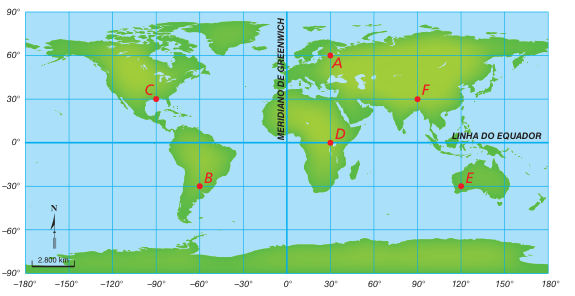
\includegraphics[width=1\linewidth]{figures/2.png}
    \end{figure}

    \begin{enumerate}[I]
      \item Entre os pontos assinalados em vermelho no mapa, determine as coordenadas do ponto:
        \begin{tasks}
          \task assinalado na região que corresponde à América do Sul.
          \task assinalado na região que corresponde à África.
          \task assinalado na região que corresponde à América do Norte.
          \task assinalado na região que corresponde à China.
          \task assinalado na região que corresponde à Europa.
          \task assinalado na região que corresponde à Austrália.
        \end{tasks}
      \item Em que continente está o ponto de latitude $60^\circ$ norte e longitude $120^\circ$ leste?
    \end{enumerate}
\end{enumerate}



\end{document}
